% !TEX TS-program = pdfLaTeX+shellescape
% !TEX encoding = UTF-8 Unicode

\documentclass{standalone}
\usepackage{pgfplots}
\pgfplotsset{compat=1.17}

\definecolor{tab_blue}{HTML}{1F77B4}
\definecolor{tab_orange}{HTML}{FF7F0E}
\definecolor{tab_green}{HTML}{2CA02C}
\definecolor{tab_red}{HTML}{D62728}

\begin{document}
    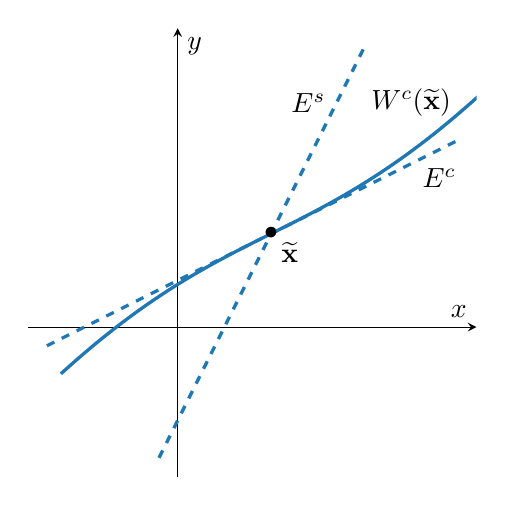
\begin{tikzpicture}[baseline]
        \begin{axis}[
            scale=1.0, % scale
            xmin=-0.8,xmax=1.6,ymin=-0.8,ymax=1.6, % range of plot
            % legend style={at={(axis cs: 1,0)}, anchor=south east}, % position of legends
            unit vector ratio = {1, 1}, % aspect ratio
            axis lines = middle, % middle or box
            %axis x line = bottom, % top, middle, bottom, none: axis x line* = ... removes arrow heads
            %axis y line = left, % left, center, right, none: axis y line* = ... removes arrow heads
            xlabel = {$x$}, ylabel = {$y$}, % axis labels 
            xtick = {10},
            ytick = {10},
        ]
            % \addplot[tab_blue, domain=-1.5:0.0, samples=100, very thick] (x, {0});   
            % \addplot[tab_blue, domain=-0.25:1.5, samples=100, very thick] ({x}, {sqrt((1+sqrt(1+4*x))/2)}); 
            % \addplot[tab_blue, domain=-0.25:0, samples=100, very thick, dashed] ({x}, {sqrt((1-sqrt(1+4*x))/2)});   
            % \addplot[tab_blue, domain=0.0:1.5, samples=100, very thick, dashed] {0};
            % \addplot[tab_blue, domain=-0.25:1.5, samples=100, very thick] ({x}, {-sqrt((1+sqrt(1+4*x))/2)});   
            % \addplot[tab_blue, domain=-0.25:0, samples=100, very thick, dashed] ({x}, {-sqrt((1-sqrt(1+4*x))/2)});   
            \addplot[tab_blue, domain=-0.7:1.5, samples=3, very thick, dashed] ({x}, {x/2 + 0.25});   
            \addplot[tab_blue, domain=-0.1:1.0, samples=3, very thick, dashed] ({x}, {2*x - 0.5}); 
            \addplot[tab_blue, domain=-0.5:0.5, samples=100, very thick] ({2*x + x^3 + 0.5}, {x + 2*x^3 + 0.5});
            \node at (0.5, 0.5) {$\bullet$};
            \node at (0.6, 0.4) {$\widetilde{\mathbf{x}}$};
            \node at (1.4, 0.8) {$E^c$}; 
            \node at (0.7, 1.2) {$E^s$}; 
            \node at (1.25, 1.2) {$W^c(\widetilde{\mathbf{x}})$};
            % \node at (2.2, 3.7) {$r>0$};
            % \node at (2.2, 2.7) {$r<0$};
            % \node[tab_blue] at (1.0, -1/6) {$\bullet$};
            % \addplot3[red, thick, domain=90:300, samples=60, samples y=1]({0.8*sin(x)}, {0.8*cos(x)}, {0});
            % \addplot3[red, variable=\t, samples=7, samples y=1, domain=110:300, -latex, quiver={u={cos(t)}, v={-sin(t)}, scale arrows=0.01}]({0.8*sin(t)}, {0.8*cos(t)}, {0});
        \end{axis}
    \end{tikzpicture}

    \begin{tikzpicture}[baseline]
        \begin{axis}[
            scale=1.0, % scale
            xmin=-0.5,xmax=0.5,ymin=-0.5,ymax=0.5, % range of plot
            % legend style={at={(axis cs: 1,0)}, anchor=south east}, % position of legends
            unit vector ratio = {1, 1}, % aspect ratio
            axis lines = middle, % middle or box
            %axis x line = bottom, % top, middle, bottom, none: axis x line* = ... removes arrow heads
            %axis y line = left, % left, center, right, none: axis y line* = ... removes arrow heads
            xlabel = {$x_c$}, ylabel = {$x_s$}, % axis labels 
            xtick = {10},
            ytick = {10},
        ]
            % \addplot[tab_blue, domain=-1.5:0.0, samples=100, very thick] (x, {0});   
            % \addplot[tab_blue, domain=-0.25:1.5, samples=100, very thick] ({x}, {sqrt((1+sqrt(1+4*x))/2)}); 
            % \addplot[tab_blue, domain=-0.25:0, samples=100, very thick, dashed] ({x}, {sqrt((1-sqrt(1+4*x))/2)});   
            % \addplot[tab_blue, domain=0.0:1.5, samples=100, very thick, dashed] {0};
            % \addplot[tab_blue, domain=-0.25:1.5, samples=100, very thick] ({x}, {-sqrt((1+sqrt(1+4*x))/2)});   
            % \addplot[tab_blue, domain=-0.25:0, samples=100, very thick, dashed] ({x}, {-sqrt((1-sqrt(1+4*x))/2)});   
            \addplot[tab_blue, domain=-0.45:0.45, samples=100, very thick] ({x}, {x^3});
            \node at (0, -0.13) {$W^c(\mathbf{0}) = \{(x_c, x_s): x_s = h_s(x_c)\}$};
            % \node at (0.5, 0.5) {$\bullet$};
            % \node at (0.6, 0.4) {$\widetilde{\mathbf{x}}$};
            % % \node at (2.2, 3.7) {$r>0$};
            % \node at (2.2, 2.7) {$r<0$};
            % \node[tab_blue] at (1.0, -1/6) {$\bullet$};
            % \addplot3[red, thick, domain=90:300, samples=60, samples y=1]({0.8*sin(x)}, {0.8*cos(x)}, {0});
            % \addplot3[red, variable=\t, samples=7, samples y=1, domain=110:300, -latex, quiver={u={cos(t)}, v={-sin(t)}, scale arrows=0.01}]({0.8*sin(t)}, {0.8*cos(t)}, {0});
        \end{axis}
    \end{tikzpicture}
\end{document}